\documentclass{article}
\usepackage{amssymb}
\usepackage{amsmath}
\usepackage{tikz}
\usepackage{pgfplots}

\usepackage{listings}
\usepackage{color}

\usepackage{pdfpages}

\definecolor{codegreen}{rgb}{0,0.6,0}
\definecolor{codegray}{rgb}{0.5,0.5,0.5}
\definecolor{codepurple}{rgb}{0.58,0,0.82}
\definecolor{backcolour}{rgb}{0.95,0.95,0.92}

\lstdefinestyle{mystyle}{
   backgroundcolor=\color{backcolour},
   commentstyle=\color{codegreen},
   keywordstyle=\color{magenta},
   numberstyle=\tiny\color{codegray},
   stringstyle=\color{codepurple},
   basicstyle=\footnotesize,
   breakatwhitespace=false,
   breaklines=true,
   captionpos=b,
   keepspaces=true,
   numbers=left,
   numbersep=5pt,
   showspaces=false,
   showstringspaces=false,
   showtabs=false,
   tabsize=2
}

\lstset{style=mystyle}

\begin{document}

\begin{flushleft}
  Eli Schmitter
\end{flushleft}
\section{R8.4}
A public interface of a class is what you can access out side of the class. An implementation of a class has private interface as well as a public interface.
\section{R8.8}
A mutator method is a method that takes a instance variable and modifies it some how, like setting it to a value. An accessor method is a method that returns an private insistence variable.

\section{R8.11}
A constructor is a method that runs at the initialization of an instance of a class.
\section{R8.14}
last two pages
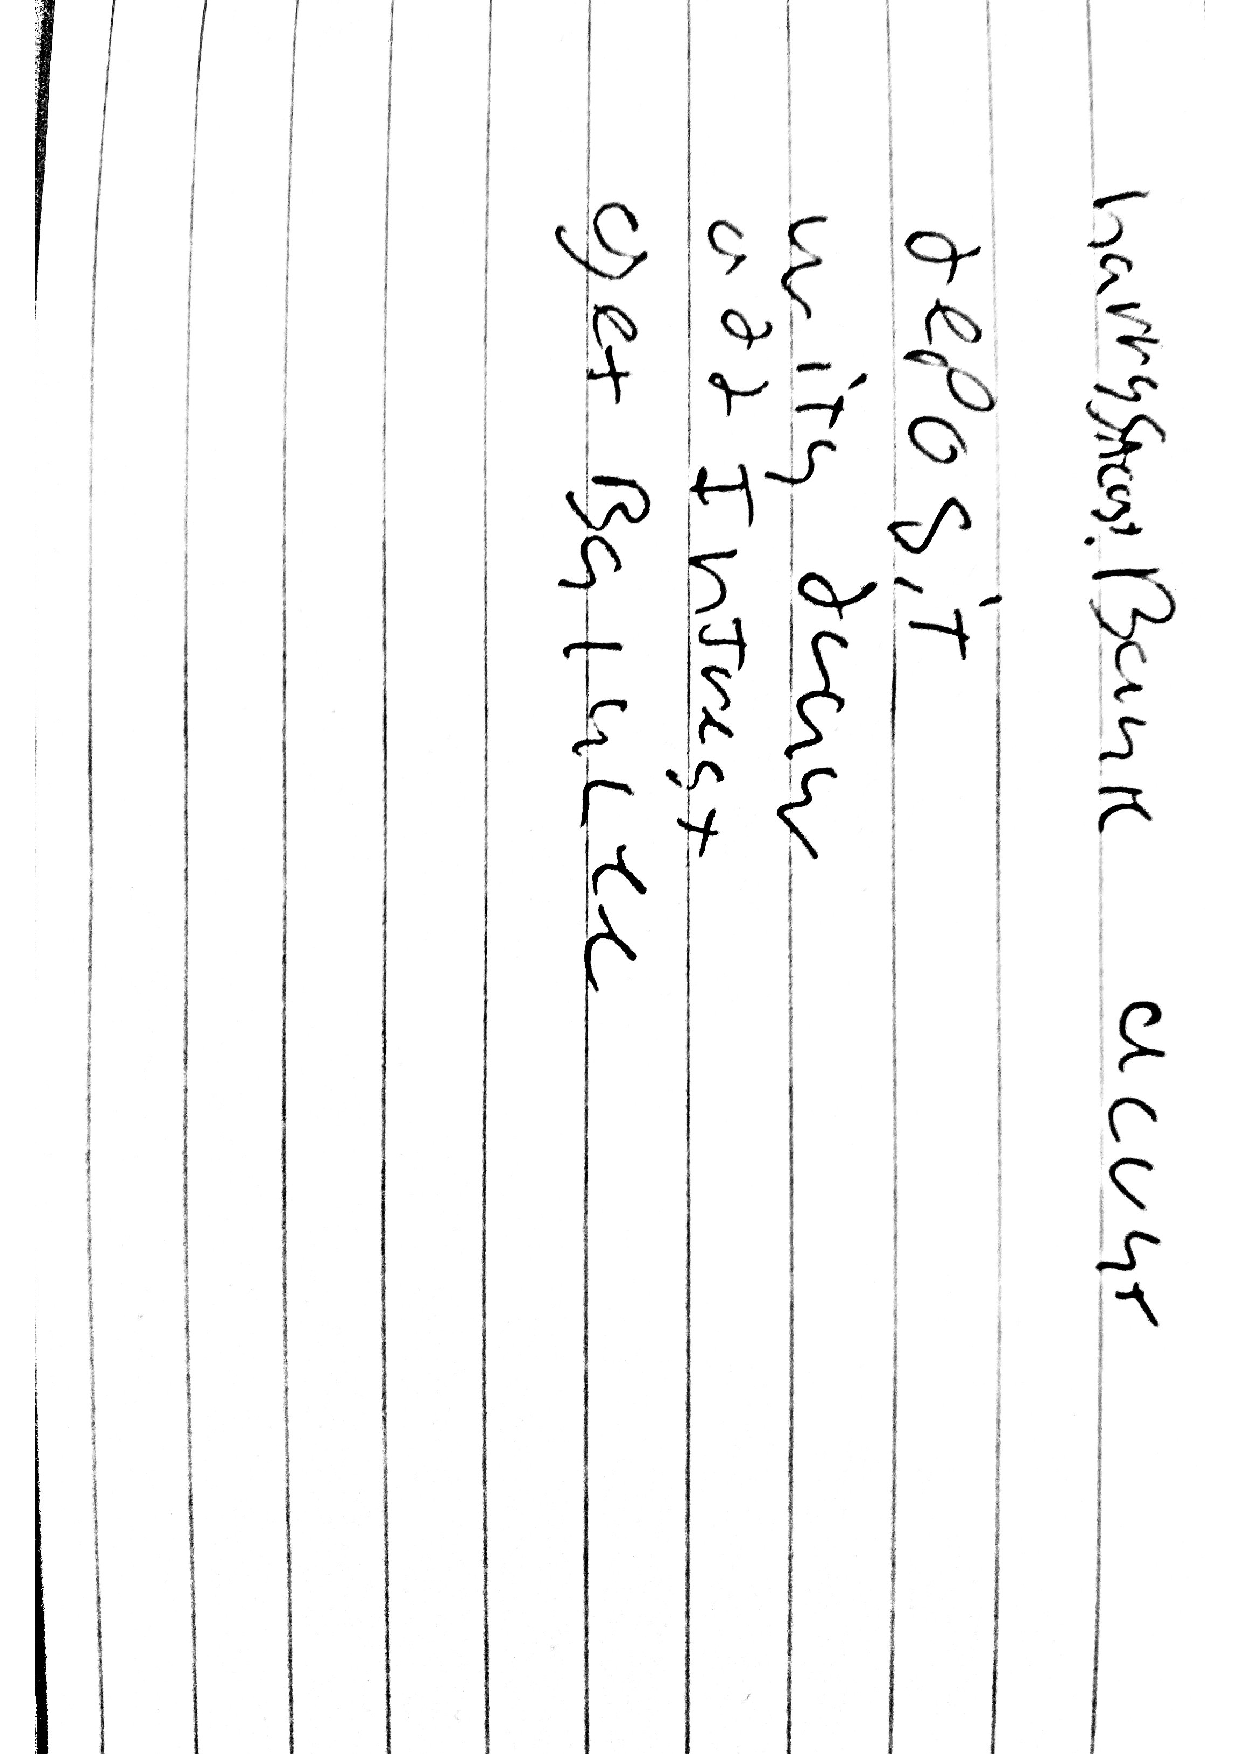
\includepdf[page={1,2}]{New}
\end{document}
